\documentclass[conference]{IEEEtran}
\IEEEoverridecommandlockouts
\usepackage{cite}
\usepackage{amsmath,amssymb,amsthm}
\usepackage{algorithm}
\usepackage[noend]{algpseudocode}
\usepackage{graphicx}
\usepackage{booktabs}
\usepackage{xcolor}
\usepackage{tikz}
\usepackage[hidelinks]{hyperref}
\usepackage{url}
\graphicspath{{../common/figures/}}
\newcommand{\code}[1]{\texttt{#1}}
\newcommand{\prop}[1]{\textsf{#1}}
\newtheorem{definition}{Definition}
\newtheorem{theorem}{Theorem}
\newtheorem{proposition}{Proposition}

\begin{document}

\title{Acceptance Semantics for MAVLink~2 Signing:\\ Bounded Symbolic Analysis and Model-Based\\ Conformance Testing of Flight Stacks}

\author{\IEEEauthorblockN{Ian Brighouse}
\IEEEauthorblockA{\textit{Brighouse Security Labs}, Spain \\ research@brighousesec.com}}
\maketitle

\begin{abstract}
The MAVLink~2 message-signing specification fixes a frame format and a timestamp
rule but delegates the decisive question---\emph{when is an unsigned or
unexpected frame accepted?}---to each implementation. The result is a family of
subtly different receivers whose security cannot be compared by reading the
specification. We give a precise, parameterised \emph{acceptance semantics} for
MAVLink~2 signing as a labelled transition system, in which the choices the
specification leaves open become explicit policy parameters, and we equip it with
a bounded symbolic adversary and six security properties with machine-checkable
definitions. Bounded breadth-first exploration is \emph{sound} (every reported
violation is a concrete trace) and \emph{complete up to a depth bound relative
to the adversary's restricted move set}; it
separates an idealised out-of-band provisioning policy, which satisfies every
property while remaining functional, from the policies PX4 and ArduPilot
implement, each of which violates a distinct subset. We then use the model
generatively: a design-space search over single parameter edits, constrained to
preserve a liveness (functionality) property, yields greedy-minimal
remediations---and shows, for example, that the current ArduPilot policy
requires \emph{two} independent changes where PX4~v1.18 requires one. Finally,
we introduce \emph{model-based conformance testing} for flight stacks: read-only
test frames derived from the semantics are executed against real
software-in-the-loop builds, and the observed accept/reject decisions are
compared with the model's predictions. In a recorded experiment across three
stacks and four link configurations the model agrees with all $47$ observed
decisions, and one configuration resolves a disagreement between a stack's
documentation and its behaviour in favour of the behaviour; we are explicit that the $20$ unkeyed cases are tautological and that
the signing-less PX4~v1.17 stack serves as a negative control, so the
discriminating evidence rests on the $23$ keyed cases, including seven observed
rejections. One pair of configurations is a controlled experiment rather than a
coincidence of agreement: moving the \emph{same} transport between channel
indices flips the decision exactly as the policy's trusted-link parameter
predicts. All
models, proofs-in-code, and harnesses are released.
\end{abstract}

\begin{IEEEkeywords}
formal methods, protocol security, transition systems, bounded model checking,
conformance testing, MAVLink, UAV security.
\end{IEEEkeywords}

\section{Introduction}
A security protocol whose acceptance rule is ``left to the implementation'' is
really a \emph{family} of protocols. MAVLink~2 message signing is such a case:
the specification pins the signature construction and a one-minute replay window
but states that acceptance of unsigned traffic ``depends on the
implementation,'' and offers only informal suggestions (accept
\code{RADIO\_STATUS}; an ``unsigned mode''; ``accept unsigned until the first
signed packet''). Two widely deployed receivers, PX4 and ArduPilot, resolve these
degrees of freedom differently, and companion measurement
work~\cite{brighouse2026signing} shows the differences have real consequences,
including a link that signs every outbound frame yet still accepts unsigned
commands. What has been missing is a \emph{model}: a precise object in which the
choices are explicit, the adversary is fixed, and the properties are stated
formally, so that implementations can be compared, attacked, and repaired by
construction.

\noindent\textbf{Contributions.}
\begin{itemize}
\item A parameterised acceptance semantics for MAVLink~2 signing
(Section~\ref{sec:sem}): a transition system whose policy parameters capture
exactly the specification's open choices, including out-of-band vs.\ over-the-wire
key provisioning.
\item A bounded symbolic adversary and six properties
(Section~\ref{sec:adv}) with a soundness result and depth-bounded completeness
(Section~\ref{sec:analysis}); exploration separates an idealised policy from the
implemented ones.
\item A generative use of the model (Section~\ref{sec:synth}): a
liveness-constrained design-space search that computes \emph{greedy-minimal}
remediations per policy (reporting ties as alternatives), yielding non-obvious
results (ArduPilot needs two independent fixes; PX4~v1.18 one).
\item Model-based conformance testing for flight stacks
(Section~\ref{sec:conf}): read-only tests derived from the semantics, executed
against real SITL builds as a recorded experiment ($47$ decisions, three stacks
and four link configurations), checking the policies against the running code.
One pair of configurations varies a single parameter---which channel index
carries a given transport---and the stack's decision flips as the policy
predicts, which separates a model of the mechanism from mere agreement.
\end{itemize}

\section{Acceptance Semantics}
\label{sec:sem}

\begin{definition}[Configuration]
A configuration is $\sigma=(K,\mathit{armed},S,\mathrm{clk})$ with key
$K\in\mathcal{K}\cup\{\bot\}$, arming flag $\mathit{armed}$, a partial map $S$
from streams $s=(\mathit{sys},\mathit{comp},\mathit{id})$ to timestamps, and a
local clock $\mathrm{clk}\in\mathbb{N}$.
\end{definition}

\begin{definition}[Frame]
A frame is $f=(\ell,\mathit{src},\kappa,b,k,t,\mathit{id})$ with link
$\ell\in\mathcal{L}$, source $\mathit{src}$, kind
$\kappa\in\{\textsc{cmd},\textsc{read},\textsc{hb},\textsc{radio},\textsc{setup}\}$,
signed bit $b\in\mathbb{B}$, signing key $k$, timestamp $t$, link id
$\mathit{id}$, and (for \textsc{setup}) a payload key $k'$. Under the standard
symbolic abstraction, $f$ \emph{verifies} in $\sigma$ iff $b$ and $k=K$:
signatures are unforgeable and collision-free.
\end{definition}

\begin{definition}[Policy]
A policy $\pi$ is a tuple
$\langle \mathsf{trusted}\subseteq\mathcal{L},\ \mathsf{allow}\subseteq
\text{Kinds},\ \mathsf{openUnkeyed},\ \mathsf{tofu},\ \mathsf{oob},\
\mathsf{uRekey},\ \mathsf{sRekey},\ \mathsf{refuseArmed},\ \mathsf{replay}\rangle$
of the specification's open choices.
\end{definition}

The transition relation $\sigma \xrightarrow{f/d}_\pi \sigma'$, with
$d\in\{\mathsf{acc},\mathsf{rej}\}$, is defined by Algorithm~1 of
\cite{brighouse2026signing} extended with the out-of-band case: when
$\mathsf{oob}$ holds the key is factory-installed, so the initial configuration
has $K\neq\bot$ and no \textsc{setup} frame is ever needed. Freshness is
$\mathrm{fresh}(\sigma,f)\equiv \neg\mathsf{replay}\lor (S(s)\!\uparrow \land\,
t+W\ge\mathrm{clk})\lor(S(s)\!\downarrow\land\,t>S(s))$ with $W=6{\times}10^6$.

We instantiate five policies (Table~\ref{tab:pol}): \textsf{spec-strict}
(strictest reading of the text), \textsf{ideal-oob} (out-of-band keys, no TOFU),
and the three measured policies \textsf{px4-1.17}, \textsf{px4-1.18},
\textsf{ardupilot-4.7.2}.

\begin{table}[t]
\caption{Policies (abridged; see \cite{brighouse2026signing} for the full tuple).}
\label{tab:pol}
\centering\footnotesize\setlength{\tabcolsep}{3pt}
\begin{tabular}{@{}lccccc@{}}
\toprule
 & trusted & TOFU & oob & u-rekey & allow \\
\midrule
\textsf{spec-strict}     & $\emptyset$ & yes & no  & no  & \{radio\}\\
\textsf{ideal-oob}       & $\emptyset$ & no  & yes & no  & \{radio\}\\
\textsf{px4-1.18}        & $\emptyset$ & yes & no  & no  & \{hb,radio\}\\
\textsf{px4-1.17}        & all         & no  & no  & --- & ---\\
\textsf{ardupilot-4.7.2} & \{ch0\}     & yes & no  & yes & \{radio\}\\
\bottomrule
\end{tabular}
\end{table}

\section{Adversary and Properties}
\label{sec:adv}

\begin{definition}[Adversary]
The adversary $A$ controls one link $a$. Its one-step moves are: inject any
unsigned frame on $a$; replay any frame previously observed on $a$; and inject a
frame signed with a key $k\in\mathit{known}(A)$. $A$ cannot forge. Keys enter
$\mathit{known}(A)$ exactly when $A$ observes a \textsc{setup} frame on $a$
(\textsc{setup} carries $k'$ in clear).
\end{definition}

Properties are predicates over reachable traces. \prop{P1}
command-integrity: no accepted \textsc{cmd} originates from $A$ on a link
$\notin\mathsf{trusted}$. \prop{P2} key-integrity: no reachable configuration has
$K=K_{\mathrm{adv}}$. \prop{P3} replay-resistance: no previously accepted
\textsc{cmd} is accepted again. \prop{P4} first-use window: $\exists$ a
pre-provisioning trace installing $K_{\mathrm{adv}}$. \prop{P5} trusted-link
exemption: $\exists$ an accepted $A$-\textsc{cmd} on a link
$\in\mathsf{trusted}$. \prop{P6} key exposure: with $A$ on the provisioning link,
$\exists$ an accepted $A$-\textsc{cmd} after key leak. \prop{P1}--\prop{P3} are
safety failures; \prop{P4}--\prop{P6} are exposure facts. Liveness
\prop{L}: a legitimately provisioned vehicle accepts a legitimate signed
\textsc{cmd} on an ordinary link.

\section{Bounded Symbolic Analysis}
\label{sec:analysis}

We explore, per policy and per scenario, all adversary action sequences up to
depth $k$ by breadth-first search, recording the shortest witness for each
property.

\begin{proposition}[Soundness]
Every witness returned is a valid trace of $\xrightarrow{}_\pi$: the reported
violation is realisable by the stated adversary.
\end{proposition}
\begin{proof}[Proof sketch]
Each search edge applies $\mathrm{step}_\pi$ to a reachable configuration and an
adversary-constructible frame; the witness is the concatenation of these edges,
hence a trace. $A$-constructibility is enforced by the move generator
(unsigned always; signed only with $k\in\mathit{known}(A)$; replay only of
observed frames). \end{proof}

\begin{proposition}[Depth-bounded completeness, relative to the move set]
Let $M$ be the adversary's move set actually generated by the exploration: frames
with a fixed adversary source identity, a fixed link identifier, and one canonical
fresh timestamp per step (the adversary does not spoof the GCS system id, vary the
link id, or choose timestamps inside the acceptance window). If a property is
violable within $k$ adversary steps \emph{drawn from $M$} from a scenario's initial
configuration (pre-, on-, or post-provisioning, as defined for that property),
the search finds a witness of length $\le k$.
\end{proposition}
\begin{proof}[Proof sketch]
For each scenario the search starts from that scenario's initial configuration;
BFS over the finitely-branching move relation enumerates all adversary sequences
of length $\le k$ over $M$. The abstraction makes the per-step frame set finite
(bounded kinds, links, keys, and a canonical fresh timestamp), so no violating
sequence of length $\le k$ over $M$ is missed. The proposition says nothing about
attacks that need moves outside $M$ (e.g.\ source-id spoofing or link-id variation
against per-stream replay state); those are future work. \end{proof}

Two caveats keep this claim honest. First, because the abstract clock advances
on every step, no two explored configurations coincide, so the visited-set in the
implementation never prunes: the search is a bounded tree enumeration, not a
closed state-space exploration. Second, the observation that $k=3$ suffices for
the measured policies is \emph{empirical}---no new property becomes violable at
$k=4$ for these policies---and is not a proven saturation. Fig.~\ref{fig:matrix}
summarises the outcome. \textsf{ideal-oob} is the unique policy with no witnessed
property in any scenario while satisfying \prop{L}; each implemented policy
violates a distinct subset, matching the measurements of
\cite{brighouse2026signing}.

\begin{figure}[t]
\centering
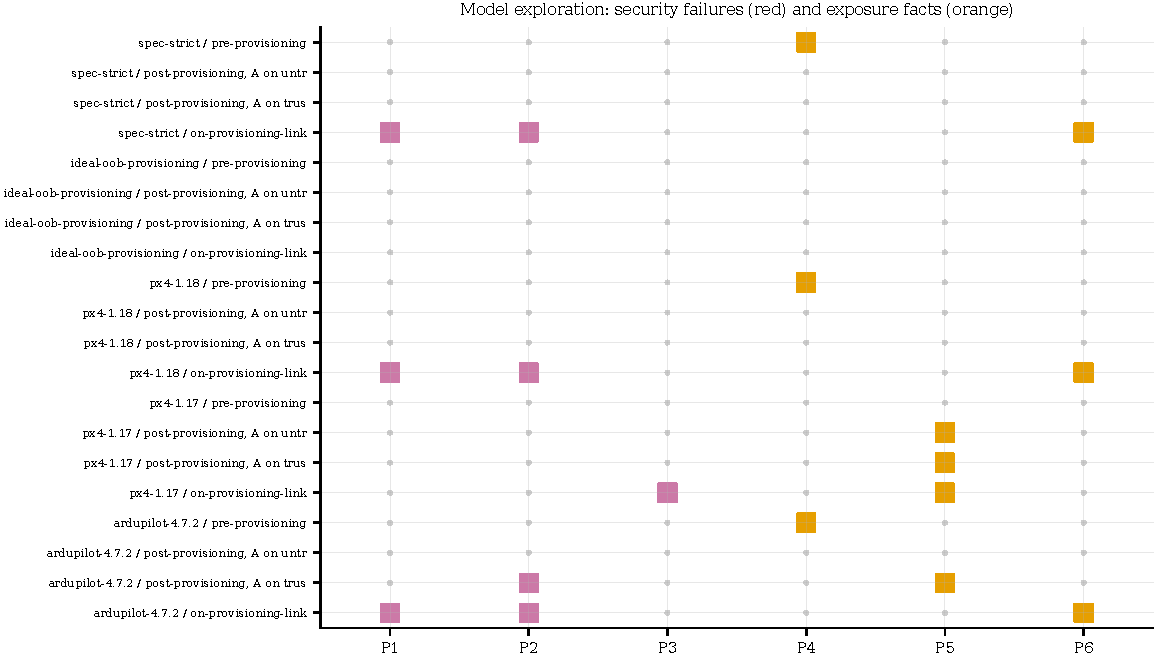
\includegraphics[width=\columnwidth]{fig_model_matrix.pdf}
\caption{Exploration ($k{=}3$). Red: safety failure witnessed; orange: exposure
fact; dot: none. \textsf{ideal-oob} is clean throughout.}
\label{fig:matrix}
\end{figure}

\section{Generative Use: Minimal Remediation}
\label{sec:synth}

Because policies are first-class, we search the design space. For a base policy
we consider the single-parameter edits in Table~\ref{tab:edits}, recompute the
witnessed set, and retain an edit only if it preserves liveness \prop{L}. A
greedy search then builds an edit set clearing all safety failures: an edit is
added only if it strictly reduces the failure count, edits that leave a policy
unchanged are never counted, iteration order is fixed (so the result is
deterministic), and when several edits are equally good at a step all of them
are reported as alternatives. The result is \emph{greedy-minimal}; we do not
claim global minimality.

\begin{table}[t]
\caption{Greedy-minimal liveness-preserving remediation (model, $k{=}3$).}
\label{tab:edits}
\centering\footnotesize\setlength{\tabcolsep}{4pt}
\begin{tabular}{@{}lp{3.1cm}c@{}}
\toprule
policy & greedy-minimal edit set clearing \prop{P1}--\prop{P3} & \prop{L}? \\
\midrule
\textsf{spec-strict}     & close TOFU + out-of-band keys & yes \\
\textsf{px4-1.18}        & close TOFU + out-of-band keys & yes \\
\textsf{ardupilot-4.7.2} & close TOFU + OOB keys \emph{and} (drop the console-link exemption \emph{or} forbid unsigned re-keying; either clears the failures) & yes \\
\textsf{px4-1.17}        & no single edit reduces the failures: adopt the full mechanism & --- \\
\textsf{ardupilot-4.7.2-doc} & no single edit reduces the failures: the MAVLink~1 downgrade keeps a forged-command path open, so closing the provisioning window no longer suffices & yes \\
\bottomrule
\end{tabular}
\end{table}

Two results are worth stating. First, closing the trust-on-first-use window is
only sound \emph{together with} out-of-band provisioning: closing TOFU alone
makes the vehicle unprovisionable (it fails \prop{L}), a trap the liveness
constraint catches automatically. Second, \textsf{ardupilot-4.7.2} requires
\emph{two} independent edits---closing the key-exposure window and removing the
unsigned re-key on the console link---because the two support distinct \prop{P2}
witnesses; \textsf{px4-1.18} requires only the first. \textsf{px4-1.17}, which
has no signing implementation, admits no small liveness-preserving fix: the whole
mechanism must be added. These are precisely the actionable recommendations a
vendor needs, derived rather than asserted.

\section{Model-Based Conformance Testing}
\label{sec:conf}

A policy in Table~\ref{tab:pol} is a \emph{hypothesis} about an implementation.
We test it. From the semantics we derive read-only probe frames---a
\code{PARAM\_REQUEST\_READ} (kind \textsc{read}) signed or unsigned, on a trusted
and an untrusted link, in the unkeyed and keyed states---and the reversible
key-management steps. For a running SITL build we execute each probe, observe
whether the vehicle responds, and compare with $\mathrm{step}_\pi$'s prediction
(Algorithm~\ref{alg:conf}). No state-changing command is ever sent.

\begin{algorithm}[t]
\caption{Conformance of policy $\pi$ to a live stack}
\label{alg:conf}
\small
\begin{algorithmic}[1]
\State $A\gets 0,\;T\gets 0$
\ForAll{$(\text{keyed},\ell,b)\in\{0,1\}\times\{\text{trust},\text{untrust}\}\times\{0,1\}$}
  \State ensure vehicle in state keyed (provision once over trusted link)
  \State $o\gets$ send unsigned/signed \textsc{read} on $\ell$; observe reply
  \State $p\gets \mathrm{step}_\pi(\sigma_{\text{keyed},\ell},\textsc{read}_b).d$
  \State $A\gets A+[o{=}p];\;T\gets T+1$
\EndFor
\State \Return agreement $A/T$ and the disagreeing cases
\endgraf
\end{algorithmic}
\end{algorithm}

Agreement turns a documentation-derived policy into a \emph{measured} one; a
disagreement is a finding about the model or the implementation.
Table~\ref{tab:conf} reports the agreement over two campaigns: three stacks in
their default link layout (eight decisions each) and four link configurations of
ArduPilot~4.7.2 in which we vary the transport of each channel. The model agrees
with all $47$ recorded decisions. That headline must be read with its evidential
weight. Twenty \emph{unkeyed} cases are tautological: with no key installed
nothing can reject, so model and stack trivially agree. The four keyed
\textsf{px4-1.17} cases are a \emph{negative control}: the policy encodes
``signing absent'' and the stack has no signing, so agreement confirms the
absence of a mechanism, not a model of one. The discriminating evidence is the
remaining $23$ keyed cases, and in particular the seven observed
\emph{rejections} (\textsf{px4-1.18}: unsigned on the trusted and on the
untrusted link; \textsf{ardupilot-4.7.2}: unsigned on the untrusted link in each
of the four configurations).

\paragraph*{A controlled pair, not merely agreement} Agreement alone cannot
distinguish a model that captures the mechanism from one that happens to predict
the same outcome. Configurations~B and~C differ in exactly one respect: which
channel index carries the UDP link. In~B the UDP link is \code{ch0} and a keyed
unsigned read is answered; in~C the UDP link is \code{ch1} and the same read is
rejected. The policy parameter under test---the set of trusted links, here
$\{\code{ch0}\}$---is the only thing that can explain the flip, and it does so in
both directions. This is the strongest conformance evidence in the paper: the
implementation's exemption is keyed to the channel \emph{index}, as the model
says, and not to the link's transport, as its source comment's rationale
(``USB on ChibiOS boards'') would suggest.

\paragraph*{A disagreement between documentation and behaviour, resolved}
Configuration~D sets a port to MAVLink~1, whose frames carry no signature field
at all. ArduPilot's signing documentation states that such a port ``is not
protected'', which, read as a policy, says a keyed non-trusted port accepts
MAVLink~1 commands. The measurement says otherwise: the keyed port rejects an
unsigned MAVLink~1 read, and the probe's frames are recorded as \code{0xFE}, so
they were genuinely version~1 and not unsigned version~2 frames.\footnote{We
record the first byte actually sent for every case, because a client library may
silently upgrade a connection to MAVLink~2 on receiving a version~2 frame; an
earlier revision of our harness labelled the wire version from the
configuration rather than from the frame, and one attempted measurement against
PX4 had to be discarded for exactly this reason.}

We therefore added the wire version to the semantics as a frame attribute
($\mathit{wire}\in\{1,2\}$, with $\mathit{wire}{=}1$ structurally implying
unsigned) and the documented behaviour as a policy parameter
($\mathit{v1\_bypasses\_signing}$), and kept the documentation's reading as a
separate policy, \textsf{ardupilot-4.7.2-doc}. The parameter earns its place in
three ways. It makes the case agree \emph{for the right reason} rather than by
the channel rule alone. It adds an adversary move---inject a version~1
frame---that separates the two policies: under the implementation's policy the
move is rejected on an ordinary link, under the documentation's reading it
delivers a command. And it changes the repair cost: for
\textsf{ardupilot-4.7.2}, closing the provisioning window
(\textsf{close-tofu+oob}) removes \prop{P1}, while for the documented reading
the same edit does not, because the downgrade keeps a forged-command path open,
so the greedy search finds no single sufficient edit at all
(Table~\ref{tab:edits}).

What the parameter does \emph{not} do is change which properties ArduPilot
violates: the channel-0 exemption already violates \prop{P1} and \prop{P2} on
its own, so both readings fail the same set. The difference is in the witnesses
and in the cost of repair. We state this plainly because a parameter that
changed nothing would still be worth reporting, and this one changes less than
its security significance might suggest.

The experiment is \emph{recorded}: the SITL
runs are not re-executed in continuous integration; the repository stores the
observed decisions and a test asserts that the model reproduces them.

\begin{table}[t]
\caption{Model-vs-implementation conformance (read-only probes). Upper block:
default link layout. Lower block: ArduPilot~4.7.2 with the transport of each
channel varied; \code{ch0} is the channel the implementation exempts.}
\label{tab:conf}
\centering\footnotesize
\begin{tabular}{@{}llcc@{}}
\toprule
stack / configuration & policy & agree & keyed rej. \\
\midrule
ArduPilot 4.7.2 (default) & \textsf{ardupilot-4.7.2} & 8/8 & 1 \\
PX4 1.18.0-rc1            & \textsf{px4-1.18}        & 8/8 & 2 \\
PX4 1.17.0 (neg.\ control) & \textsf{px4-1.17}       & 8/8 & 0 \\
\midrule
A: \code{ch0} TCP, \code{ch1} TCP & \textsf{ardupilot-4.7.2} & 6/6 & 1 \\
B: \code{ch0} \textbf{UDP}, \code{ch1} TCP & \textsf{ardupilot-4.7.2} & 6/6 & 1 \\
C: \code{ch0} TCP, \code{ch1} \textbf{UDP} & \textsf{ardupilot-4.7.2} & 6/6 & 1 \\
D: \code{ch1} MAVLink~1 & \textsf{ardupilot-4.7.2} & 5/5 & 1 \\
\midrule
total & & \textbf{47/47} & 7 \\
\bottomrule
\end{tabular}
\end{table}

\section{Discussion and Related Work}
\label{sec:disc}

Our analysis is a bounded, special-purpose model checker rather than a
general-purpose symbolic prover. A ProVerif or Tamarin encoding of the signing
and provisioning sub-protocol---capturing unbounded sessions and the truncated-MAC
abstraction more faithfully---is natural future work; we provide the semantics in
a form amenable to such an encoding. The value of the lightweight model is that it
is executable, testable against implementations, and generative. Based on their published abstracts, the only prior formal work on MAVLink models
the protocol \emph{without} its native signing and verifies an external
cipher~\cite{wray2025pave,mak2025evtol},
or uses session types and runtime monitors with no
cryptography~\cite{amorim2025datum,amorim2026platum}; none models the signing
scheme itself---its truncated MAC, per-stream timestamp window, and
\textsc{setup\_signing} provisioning. Our methodological lineage is the symbolic
analysis of adjacent provisioning protocols: Tamarin for ASTM~F3411 Remote
ID~\cite{alam2026remoteid}, ProVerif for Bluetooth ``Just
Works''/passkey~\cite{wu2022bluetooth,jangid2023passkey} and Matter
commissioning~\cite{duttagupta2025matter}, and Tamarin for automotive
SecOC~\cite{bodei2024autosar}. To our knowledge, no prior work gives an
executable model of MAVLink's \emph{native} signing scheme and its provisioning
(as opposed to an added cipher or a runtime monitor), nor checks such a model by
model-based conformance testing against a flight stack's running implementation;
we state this on the basis of published abstracts and will revise it if the full
texts show otherwise.
Fuzzing of flight stacks~\cite{kim2019rvfuzzer,kim2021pgfuzz} targets input
validation, a complementary concern: our model assumes memory safety and studies
the acceptance decision.

\section{Conclusion}
Making the specification's open choices explicit turns ``MAVLink signing'' into a
comparable, attackable, repairable family of policies. Bounded symbolic analysis
separates an idealised policy from the deployed ones with concrete witnesses; a
liveness-constrained search derives greedy-minimal fixes (with equally good
alternatives made explicit) and reveals that ArduPilot needs two where PX4~v1.18
needs one; and model-based conformance testing, honestly accounted, ties the
discriminating part of the construction back to the running code.

\section*{Availability}
The executable semantics, exploration, synthesis, conformance harness, and tests
are released at the project repository.\footnote{Repository and data: \url{https://github.com/brigghouse/brighouse-autonomy-lab}} The work is defensive and uses only self-hosted simulators.

\bibliographystyle{IEEEtran}
\bibliography{../common/refs}
\end{document}
